\section{Continuously-variable Resonance Combustor}\label{sec:cvrc}

We now turn to our first reacting flow case, a model of the continuously-variable resonance combustor (CVRC) with a truncated combustion chamber. The CVRC experiment originated in work by Yu \textit{et al.}~\cite{Yu2008,Yu2009,Yu2012} at Purdue University, whereby a single-element, gaseous propellant, coaxial dump injection rocket combustor was designed to allow for continuous actuation of the oxidizer injection post. This actuation revealed that certain oxidizer post lengths gave rise to high-frequency combustion instabilities. The CVRC has become a useful numerical benchmark case for simulating rocket combustion~\cite{Garby2013,Nguyen2018} and investigating the mechanics which contribute to combustion instabilities in rocket engines~\cite{HarvazinskiCVRCOrig,Harvazinski2016,HarvazinskiCVRCflamelet}.

In this work, we do not model the full injector and combustor geometry of the CVRC, as in~\cite{HarvazinskiCVRCOrig}. Instead, as will be detailed in the following section, we neglect the oxidizer injection choke manifold and truncate the combustion chamber well downstream of the dump plane. This has the effect of decreasing computational costs, while still including much of the complex combusting flow phenomena such the mixing shear layer, recirculation of hot products, and large-scale transport and mixing in the combustion chamber. We do not apply acoustic forcing at the outlet to mimic the combustion instability as this would necessitate complex boundary treatments in any PROMs, which are beyond the scope of this work. We direct the read to work by Huang \textit{et al.}~\cite{Huang2022a} for a thorough investigation of artificial boundary forcing treatments for PROMs.

\subsection{Full-order Model}

The truncated CVRC case presented here generally follows that investigated by Harvazinski and Shimizu~\cite{HarvazinskiCVRCflamelet}, with a truncated combustion chamber. The geometry is displayed in Fig.~\ref{fig:cvrcGeom}. The oxidizer post extends approximately 14 cm usptream of the dump plane ($x = $ 0 m), with a diameter of 2.05 cm. The annular fuel injection port has an outer diameter of 23.09 cm and an inner diameter of 22.27 cm, extends 30.55 cm upstream of the dump plane, and enters the oxidizer stream 10.18 cm upstream of the dump plane. The combustion chamber has a diameter of 4.5 cm, and extends approximately 14 cm downstream of the dump plane. The oxidizer inlet injects 42.35\% gaseous oxygen and 57.65\% water vapor by mass at 1,030 K, with a specified mass flow rate of 0.32 kg/s. Gaseous methane is injected through the fuel duct at 300 K, with a mass flow rate of 0.027 kg/s. The computational mesh is composed of 2,637,771 hexahedral cells, resulting in a total number of degrees of freedom $\numDOF =$ 18,464,397. No-slip, adiabatic conditions are enforced at the domain walls, and a subsonic characteristic boundary condition is applied at the outlet.

\begin{figure}
	\centering
	\ifdefined\DRAFT
		\includegraphics[width=0.8\linewidth]{example-image-a}
	\else
    	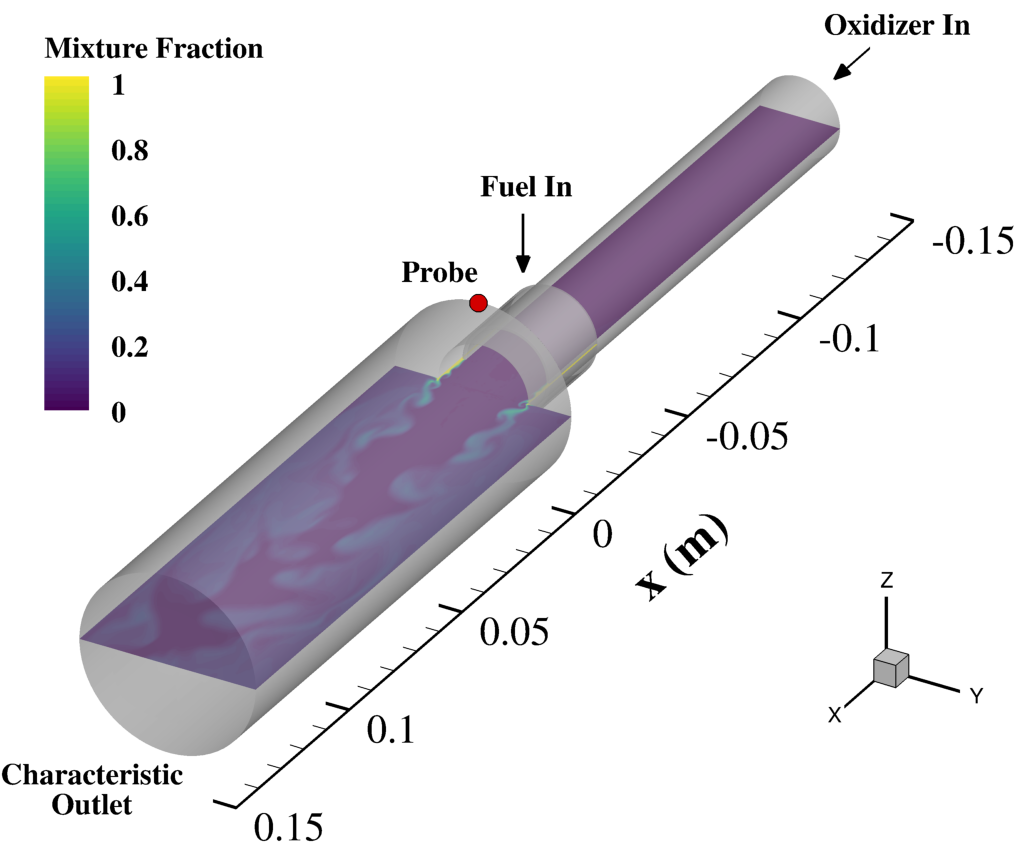
\includegraphics[width=0.8\linewidth]{Chapters/CavityAndCVRC/Images/cvrc/geom.png}
	\fi
    \caption{\label{fig:cvrcGeom}
	Truncated CVRC geometry with $x-y$ plane slice at $\timeVar = 5.6$ ms.}
\end{figure}

Combustion is modeled using the FPV approach~\cite{Pierce2001} detailed in Section~\ref{sec:fpv}. As detailed previously, a library of steady diffusion flame solutions is pre-computed off-line, generating a lookup table mapping from the mixture fraction $Z$ and the progress variable $C$ to individual species mass fractions, i.e., $Y_i = Y_i(Z,C)$. For this case, the steady flame solutions are solved using the FlameMaster software~\cite{flamemaster} with the GRI-Mech 1.2 methane combustion mechanism~\cite{griMech}. The GRI-Mech 1.2 mechanism contains 32 chemical species and 177 reactions. All gases are treated as thermally perfect gases, and thermodynamic quantities (specific heats, enthalpy, and entropy) as well as transport properties (mass diffusivity, viscosity, and thermal conductivity) are computed from polynomial functions of temperature developed by McBride et al.~\cite{McBride1993} and described in Section~\ref{subsec:gasModels}.

The FOM simulation is computed with a physical time step of $\dt = 0.1 \; \mu$s. The fluid domain is initialized with a pressure of 1 MPa, and the combustion chamber is filled with hot products at 2,000 K to initiate combustion. Initial transients exit the domain before data collection begins at 5 ms of simulation time. Data snapshots are collected over a 1 ms window, sampled every ten time steps, corresponding to roughly one flow-through time in the combustion chamber. This results in 1,001 snapshots (including the initial condition at $\timeVar =$ 5 ms) of the conservative and primitive states. Representative snapshot slices of various flow fields are displayed in Fig.~\ref{fig:cvrcFOMSlices}, using the same $x-y$ plane slice shown in Fig.~\ref{fig:cvrcGeom}.

\begin{figure}
	\begin{minipage}{0.99\linewidth}
		\ifdefined\DRAFT
			\includegraphics[width=0.99\linewidth,trim={0.0cm 3cm 0.0cm 3cm},clip]{example-image-a}
		\else
			\raisebox{-0.5\height}{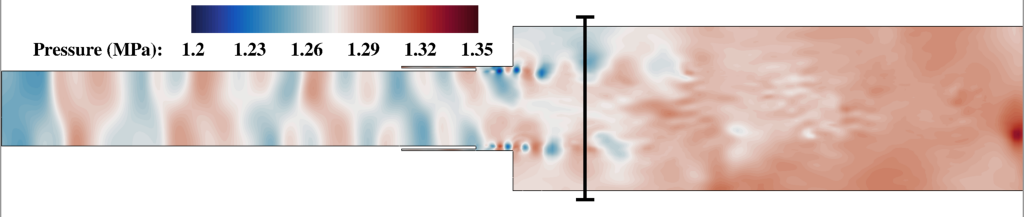
\includegraphics[width=0.84\linewidth,trim={0.2em 0.1em 0.2em 0.1em},clip]{Chapters/CavityAndCVRC/Images/cvrc/example_pressure_z.png}}
			\raisebox{-0.5\height}{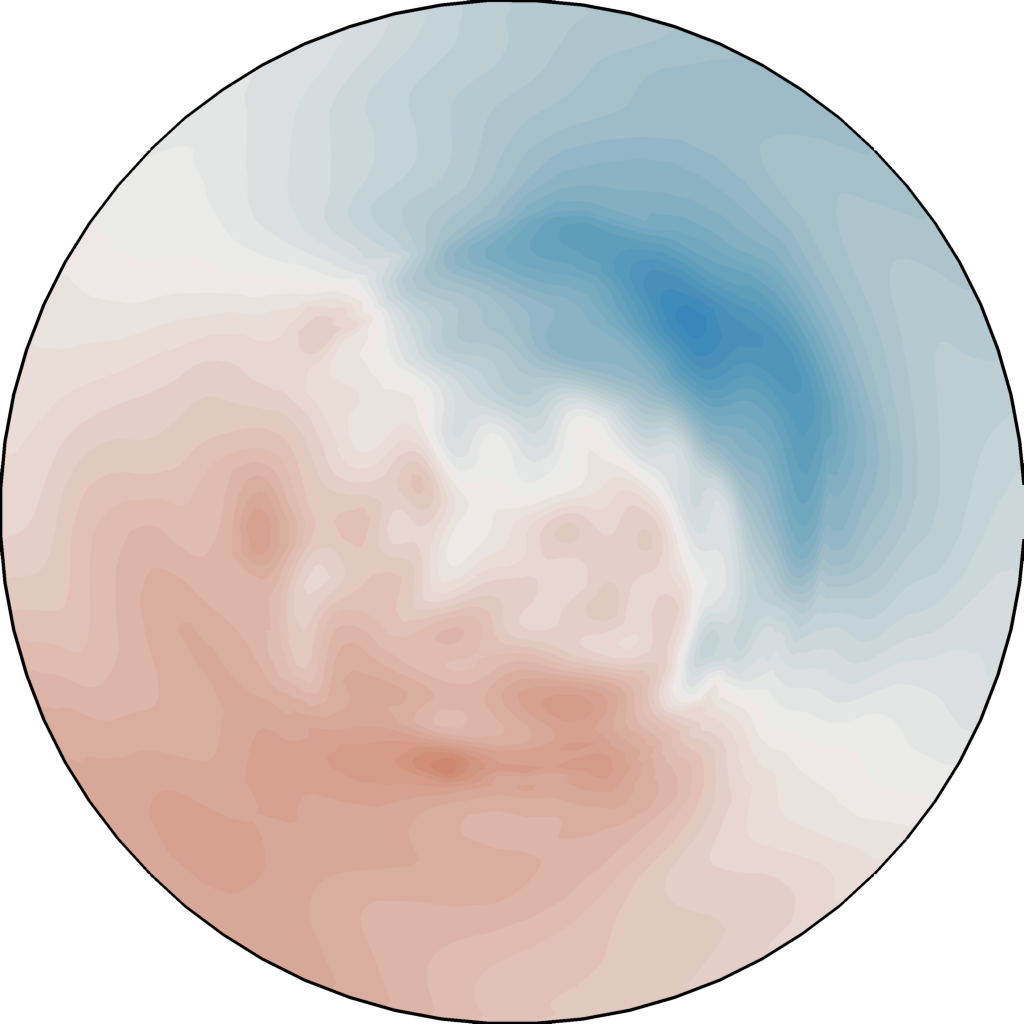
\includegraphics[width=0.14\linewidth,trim={0.0em 0.1em 0.0em 0.1em},clip]{Chapters/CavityAndCVRC/Images/cvrc/example_pressure_x.png}}
		\fi
	\end{minipage}
	\begin{minipage}{0.99\linewidth}
		\ifdefined\DRAFT
			\includegraphics[width=0.99\linewidth,trim={0.0cm 3cm 0.0cm 3cm},clip]{example-image-a}
		\else
			\raisebox{-0.5\height}{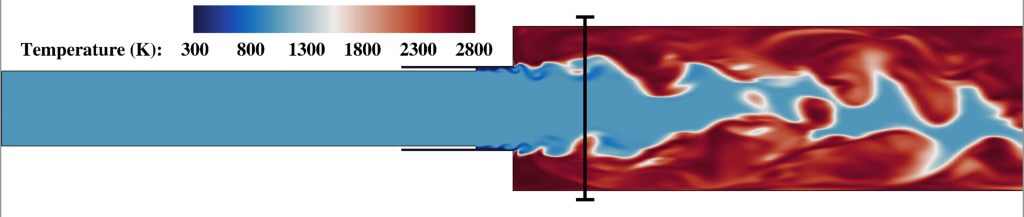
\includegraphics[width=0.84\linewidth,trim={0.2em 0.1em 0.2em 0.1em},clip]{Chapters/CavityAndCVRC/Images/cvrc/example_temperature_z.png}}
			\raisebox{-0.5\height}{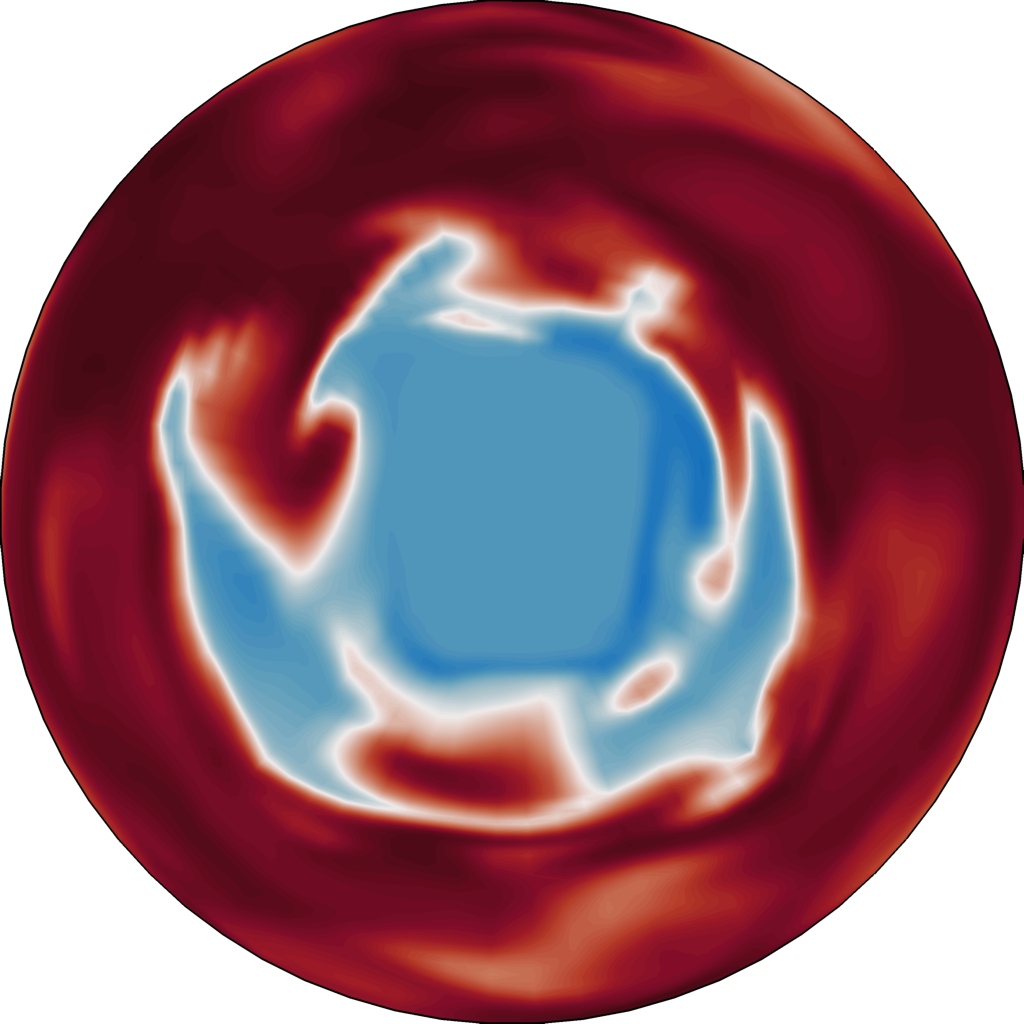
\includegraphics[width=0.14\linewidth,trim={0.0em 0.1em 0.0em 0.1em},clip]{Chapters/CavityAndCVRC/Images/cvrc/example_temperature_x.png}}
		\fi
	\end{minipage}
	\begin{minipage}{0.99\linewidth}
		\ifdefined\DRAFT
			\includegraphics[width=0.99\linewidth,trim={0.0cm 3cm 0.0cm 3cm},clip]{example-image-a}
		\else
			\raisebox{-0.5\height}{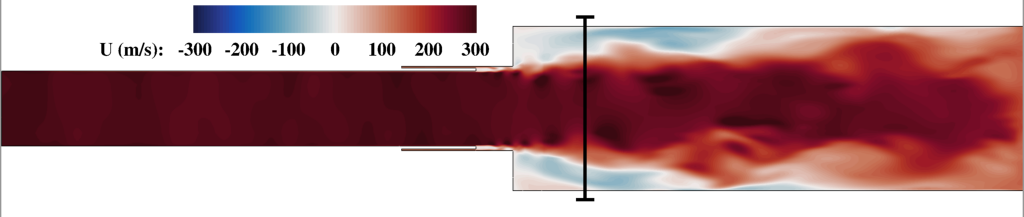
\includegraphics[width=0.84\linewidth,trim={0.2em 0.1em 0.2em 0.1em},clip]{Chapters/CavityAndCVRC/Images/cvrc/example_xVel_z.png}}
			\raisebox{-0.5\height}{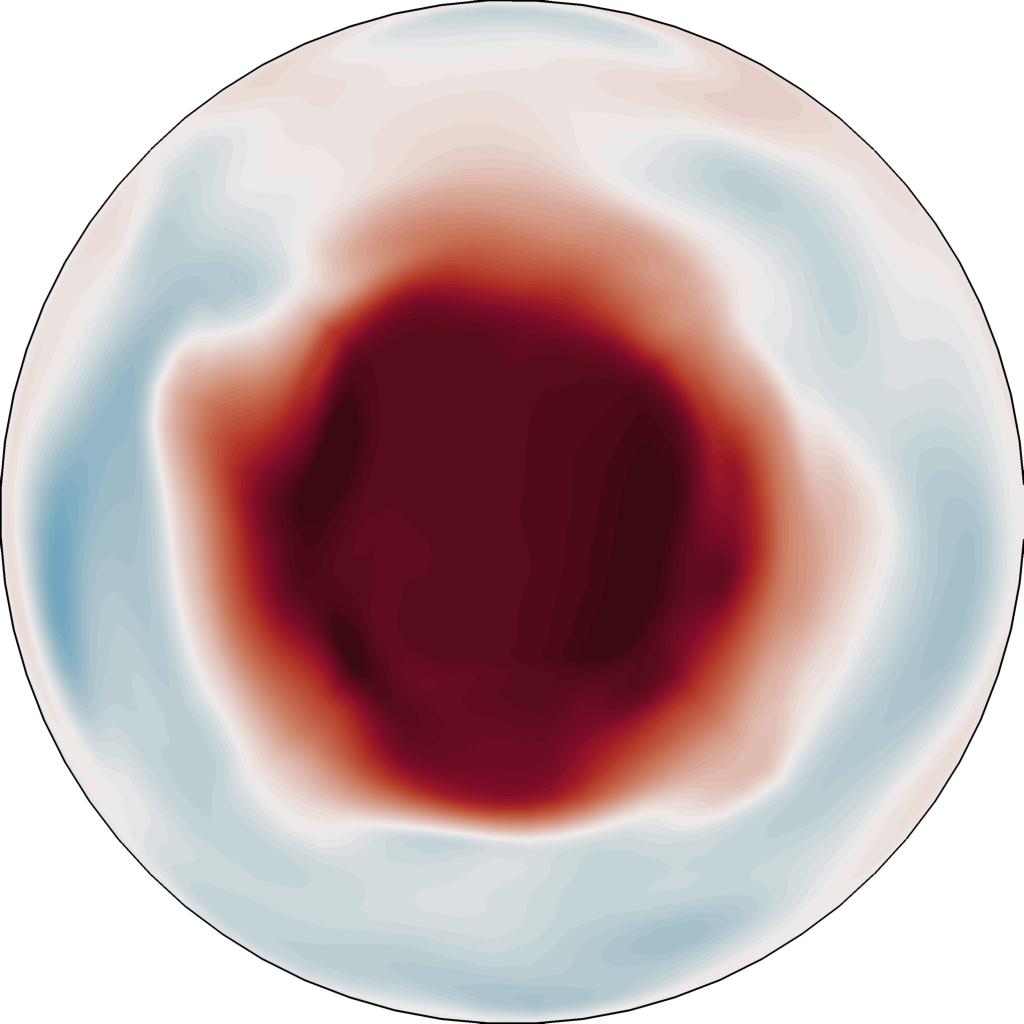
\includegraphics[width=0.14\linewidth,trim={0.0em 0.1em 0.0em 0.1em},clip]{Chapters/CavityAndCVRC/Images/cvrc/example_xVel_x.png}}
		\fi
	\end{minipage}
	\begin{minipage}{0.99\linewidth}
		\ifdefined\DRAFT
			\includegraphics[width=0.99\linewidth,trim={0.0cm 3cm 0.0cm 3cm},clip]{example-image-a}
		\else
			\raisebox{-0.5\height}{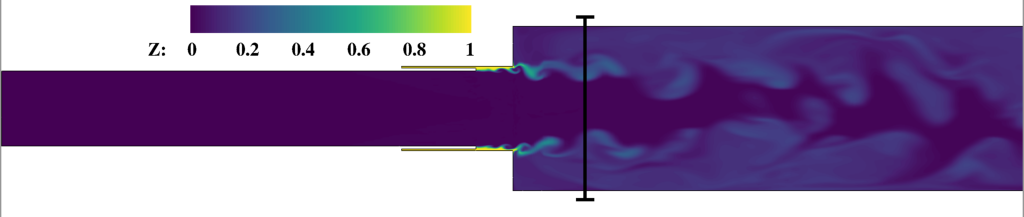
\includegraphics[width=0.84\linewidth,trim={0.2em 0.1em 0.2em 0.1em},clip]{Chapters/CavityAndCVRC/Images/cvrc/example_mixFrac_z.png}}
			\raisebox{-0.5\height}{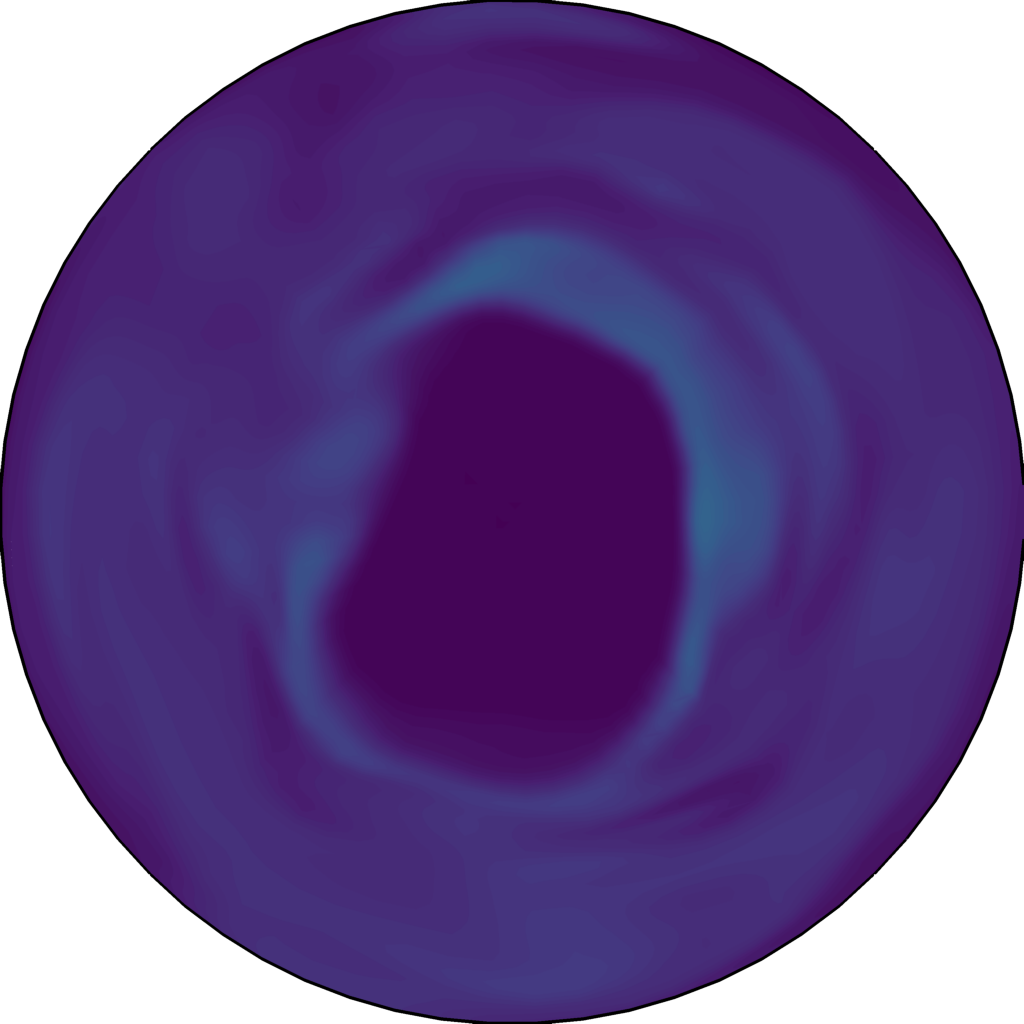
\includegraphics[width=0.14\linewidth,trim={0.0em 0.1em 0.0em 0.1em},clip]{Chapters/CavityAndCVRC/Images/cvrc/example_mixFrac_x.png}}
		\fi
	\end{minipage}
	\caption{\label{fig:cvrcFOMSlices}From top to bottom: pressure, temperature, axial velocity, and fuel mixture fraction slices at $\timeVar = 5.6$ ms.}
\end{figure}

Figure~\ref{fig:cvrcPODEnergy} displays the POD residual energy for the model rocket combustor data. Achieving 1\%, 0.1\%, and 0.01\% residual energy for the conservative dataset requires 93, 227, and 473 basis modes, respectively. For the primitive dataset, these levels require 81, 239, and 517 modes respectively. This decay is remarkably slower than that observed for 2D open cavity flow (Fig.~\ref{fig:cavityPODEnergy}), and is another of the difficult with which linear trial spaces capture the highly non-linear flow physics which characterize rocket combustion. This is further emphasized in the projection error plots shown in Figs.~\ref{fig:cvrcProjErrPrim} and~\ref{fig:cvrcProjErrCons}, where we see that radial velocity (the average of $y$- and $z$-velocity errors) induces nearly 30\% error even with 250 modes. Additionally, transported scalars exhibit high levels of error, though this improves more rapidly with trial space enrichment.

\begin{figure}
	\centering
	\ifdefined\DRAFT
		\includegraphics[width=0.8\linewidth]{example-image-a}
	\else
		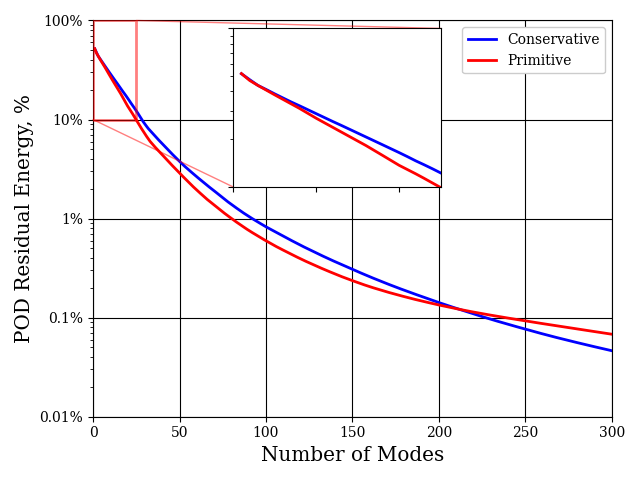
\includegraphics[width=0.8\linewidth]{Chapters/CavityAndCVRC/Images/cvrc/cvrc_pod_energy_10ms.png}
	\fi
	\caption{\label{fig:cvrcPODEnergy}POD residual energy decay for truncated CVRC conservative and primitive state datasets.}
\end{figure}

\begin{figure}
	\begin{minipage}{0.48\linewidth}
		\ifdefined\DRAFT
			\includegraphics[width=0.99\linewidth]{example-image-a}
		\else
			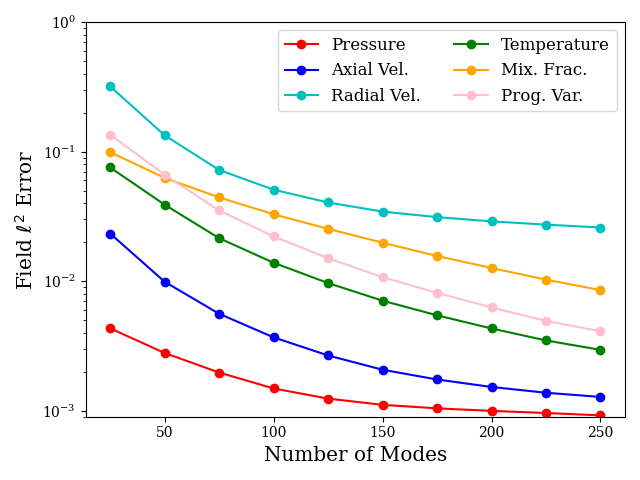
\includegraphics[width=0.99\linewidth,trim={0.5em 0.5em 0.5em 0.5em},clip]{Chapters/CavityAndCVRC/Images/cvrc/projection_error_primitive.png}
		\fi
		\caption{\label{fig:cvrcProjErrPrim}Primitive variables time-average projection error.}
	\end{minipage} \hspace{0.5em}
	\begin{minipage}{0.48\linewidth}
		\ifdefined\DRAFT
			\includegraphics[width=0.99\linewidth]{example-image-a}
		\else
			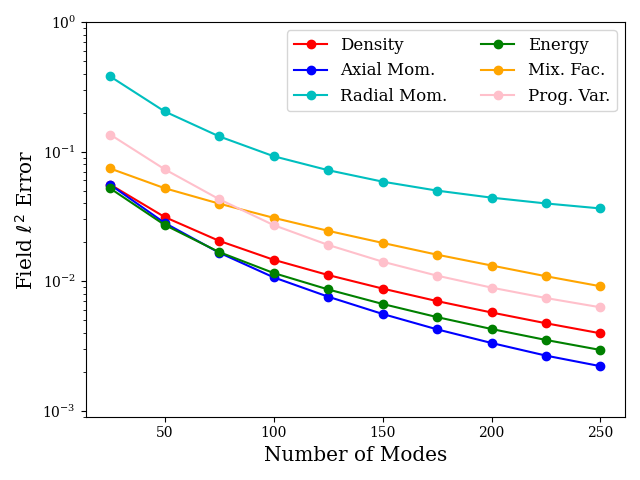
\includegraphics[width=0.99\linewidth,trim={0.5em 0.5em 0.5em 0.5em},clip]{Chapters/CavityAndCVRC/Images/cvrc/projection_error_conservative.png}
		\fi
		\caption{\label{fig:cvrcProjErrCons}Conservative variables time-average projection error.}
	\end{minipage}
\end{figure}


\subsection{Unsampled PROMs}